%% This documentation was generated with Faust version 2.6.3
%% Fri Sep 28 15:35:33 2018
%% https://faust.grame.fr

\documentclass{article}

\usepackage[utf8]{inputenc}
\usepackage{graphicx}
\usepackage[usenames]{color}
\usepackage{listings}
\usepackage{supertabular}
\usepackage{amsmath}
\usepackage{latexsym, amssymb}
\usepackage{breqn}

% No indent
\setlength{\parindent}{0pt}

% Make LaTeX output a dot when typing an asterisk
\DeclareMathSymbol{*}{\mathbin}{symbols}{"01}

% lstlistings setup
\definecolor{yobg}{rgb}{0.9,0.9,1}
\definecolor{yotxt}{rgb}{0.01,0.01,0.52} % a dark blue.
\definecolor{mylstbg}{rgb}{0.98,0.98,0.98} % a really pale grey.
\definecolor{mylstcmt}{rgb}{0.01,0.52,0.01} % a dark green.
\definecolor{mylstdoc}{rgb}{0.80,0.30,0.80} % a medium pink.

\lstset{%
  language=C++, 
  numbers=left,%none,
  tabsize=4, 
  frame=single, 
  breaklines=true, 
  numberstyle=\tiny\ttfamily, 
  backgroundcolor=\color{mylstbg}, 
  basicstyle=\scriptsize\ttfamily, 
  commentstyle=\slshape\color{mylstcmt}, %\itshape,
  frameround=tttt, 
  columns=flexible, %fixed, 
  showstringspaces=false,
  emptylines=2,
  inputencoding=utf8,
  extendedchars=true,
  literate=	{á}{{\'a}}1 
			{à}{{\`a}}1 
			{ä}{{\"a}}1 
			{â}{{\^a}}1
			{é}{{\'e}}1 
			{è}{{\`e}}1 
			{ë}{{\"e}}1 
			{ê}{{\^e}}1
			{ï}{{\"i}}1 
			{î}{{\^i}}1
			{ö}{{\"o}}1 
			{ô}{{\^o}}1
			{è}{{\`e}}1 
			{ù}{{\`u}}1 
			{û}{{\^u}}1
			{ç}{{\c{c}}}1 
			{Ç}{{\c{C}}}1,
  emph={component, declare, environment, import, library, process},
  emph={[2]ffunction, fconstant, fvariable},
  emph={[3]button, checkbox, vslider, hslider, nentry, vgroup, hgroup, tgroup, vbargraph, hbargraph, attach},
  emphstyle=\color{yotxt}, %\underline, %\bfseries,
  morecomment=[s][\color{mylstdoc}]{<mdoc>}{</mdoc>},
  rulecolor=\color{black}
}

\newcommand{\faustfilename}{src/KMH114\_channel\_map.dsp}
\newcommand{\faustdocdir}{KMH114\_channel\_map-mdoc}
\newcommand{\faustprogname}{KMH114\_channel\_map}
\newcommand{\faustversion}{2.6.3}
\newcommand{\faustdocdate}{September 28, 2018}

\begin{document}
\title{Channel mapping for Studio 114(C)} \author{ Henrik Frisk } \date{\today} \maketitle \begin{tabular}{ll}  \hline  \textbf{author} &  Henrik Frisk  \\  \textbf{basics.lib/name} & Faust Basic Element Library \\  \textbf{basics.lib/version} & 0.0 \\  \textbf{copyright} & (c) dinergy 2018  \\  \textbf{filename} & KMH114\_channel\_map \\  \textbf{license} &  BSD  \\  \textbf{maths.lib/author} & GRAME \\  \textbf{maths.lib/copyright} & GRAME \\  \textbf{maths.lib/license} & LGPL with exception \\  \textbf{maths.lib/name} & Faust Math Library \\  \textbf{maths.lib/version} & 2.1 \\  \textbf{name} & Channel mapping for Studio 114(C) \\  \textbf{version} &  0.1  \\  \hline \end{tabular} \bigskip  \bigskip This document provides a mathematical description of the Faust program text stored in the \texttt{\faustfilename} file. See the notice in Section\,\ref{notice} (page\,\pageref{notice}) for details.   \section{Mathematical definition of \texttt{process}} \label{equation}  The \emph{\faustprogname} program evaluates the signal transformer denoted by \texttt{process}, which is mathematically defined as follows: 
% Set of Faust formulas (corresponding to an <equation> tag).
\begin{enumerate}

\item Output signals $y_i$ for $i \in [1,15]$ such that
	\begin{dgroup*}
		\begin{dmath*}
				y_{1}(t) = x_{1}(t)
		\end{dmath*}
		\begin{dmath*}
				y_{2}(t) = x_{2}(t)
		\end{dmath*}
		\begin{dmath*}
				y_{3}(t) = x_{14}(t)
		\end{dmath*}
		\begin{dmath*}
				y_{4}(t) = x_{15}(t)
		\end{dmath*}
		\begin{dmath*}
				y_{5}(t) = x_{7}(t)
		\end{dmath*}
		\begin{dmath*}
				y_{6}(t) = x_{4}(t)
		\end{dmath*}
		\begin{dmath*}
				y_{7}(t) = x_{8}(t)
		\end{dmath*}
		\begin{dmath*}
				y_{8}(t) = x_{3}(t)
		\end{dmath*}
		\begin{dmath*}
				y_{9}(t) = x_{6}(t)
		\end{dmath*}
		\begin{dmath*}
				y_{10}(t) = x_{5}(t)
		\end{dmath*}
		\begin{dmath*}
				y_{11}(t) = x_{9}(t)
		\end{dmath*}
		\begin{dmath*}
				y_{12}(t) = x_{10}(t)
		\end{dmath*}
		\begin{dmath*}
				y_{13}(t) = x_{12}(t)
		\end{dmath*}
		\begin{dmath*}
				y_{14}(t) = x_{11}(t)
		\end{dmath*}
		\begin{dmath*}
				y_{15}(t) = x_{13}(t)
		\end{dmath*}
	\end{dgroup*}

\item Input signals $x_i$ for $i \in [1,15]$ 

\item Intermediate signals  $r_i$ for $i \in [1,15]$ such that
	\begin{dgroup*}
		\begin{dmath*}
				r_{1}(t) = \max\left( r_{1}(t\!-\!1) - k_{1}, \left\lvert{x_{1}(t)}\right\rvert \right)
		\end{dmath*}
		\begin{dmath*}
				r_{2}(t) = \max\left( r_{2}(t\!-\!1) - k_{1}, \left\lvert{x_{2}(t)}\right\rvert \right)
		\end{dmath*}
		\begin{dmath*}
				r_{3}(t) = \max\left( r_{3}(t\!-\!1) - k_{1}, \left\lvert{x_{14}(t)}\right\rvert \right)
		\end{dmath*}
		\begin{dmath*}
				r_{4}(t) = \max\left( r_{4}(t\!-\!1) - k_{1}, \left\lvert{x_{15}(t)}\right\rvert \right)
		\end{dmath*}
		\begin{dmath*}
				r_{5}(t) = \max\left( r_{5}(t\!-\!1) - k_{1}, \left\lvert{x_{7}(t)}\right\rvert \right)
		\end{dmath*}
		\begin{dmath*}
				r_{6}(t) = \max\left( r_{6}(t\!-\!1) - k_{1}, \left\lvert{x_{4}(t)}\right\rvert \right)
		\end{dmath*}
		\begin{dmath*}
				r_{7}(t) = \max\left( r_{7}(t\!-\!1) - k_{1}, \left\lvert{x_{8}(t)}\right\rvert \right)
		\end{dmath*}
		\begin{dmath*}
				r_{8}(t) = \max\left( r_{8}(t\!-\!1) - k_{1}, \left\lvert{x_{3}(t)}\right\rvert \right)
		\end{dmath*}
		\begin{dmath*}
				r_{9}(t) = \max\left( r_{9}(t\!-\!1) - k_{1}, \left\lvert{x_{6}(t)}\right\rvert \right)
		\end{dmath*}
		\begin{dmath*}
				r_{10}(t) = \max\left( r_{10}(t\!-\!1) - k_{1}, \left\lvert{x_{5}(t)}\right\rvert \right)
		\end{dmath*}
		\begin{dmath*}
				r_{11}(t) = \max\left( r_{11}(t\!-\!1) - k_{1}, \left\lvert{x_{9}(t)}\right\rvert \right)
		\end{dmath*}
		\begin{dmath*}
				r_{12}(t) = \max\left( r_{12}(t\!-\!1) - k_{1}, \left\lvert{x_{10}(t)}\right\rvert \right)
		\end{dmath*}
		\begin{dmath*}
				r_{13}(t) = \max\left( r_{13}(t\!-\!1) - k_{1}, \left\lvert{x_{12}(t)}\right\rvert \right)
		\end{dmath*}
		\begin{dmath*}
				r_{14}(t) = \max\left( r_{14}(t\!-\!1) - k_{1}, \left\lvert{x_{11}(t)}\right\rvert \right)
		\end{dmath*}
		\begin{dmath*}
				r_{15}(t) = \max\left( r_{15}(t\!-\!1) - k_{1}, \left\lvert{x_{13}(t)}\right\rvert \right)
		\end{dmath*}
	\end{dgroup*}

\item Constant $k_1$ such that
	\begin{dgroup*}
		\begin{dmath*}
				k_{1} = \frac{1}{\min\left( 192000, \max\left( 1, f_S \right) \right)}
		\end{dmath*}
	\end{dgroup*}

\end{enumerate}

 \section{Block diagram of \texttt{process}} \label{diagram}  The block diagram of \texttt{process} is shown on Figure\,\ref{figure1} (page\,\pageref{figure1}). \begin{figure}[ht!]
	\centering
	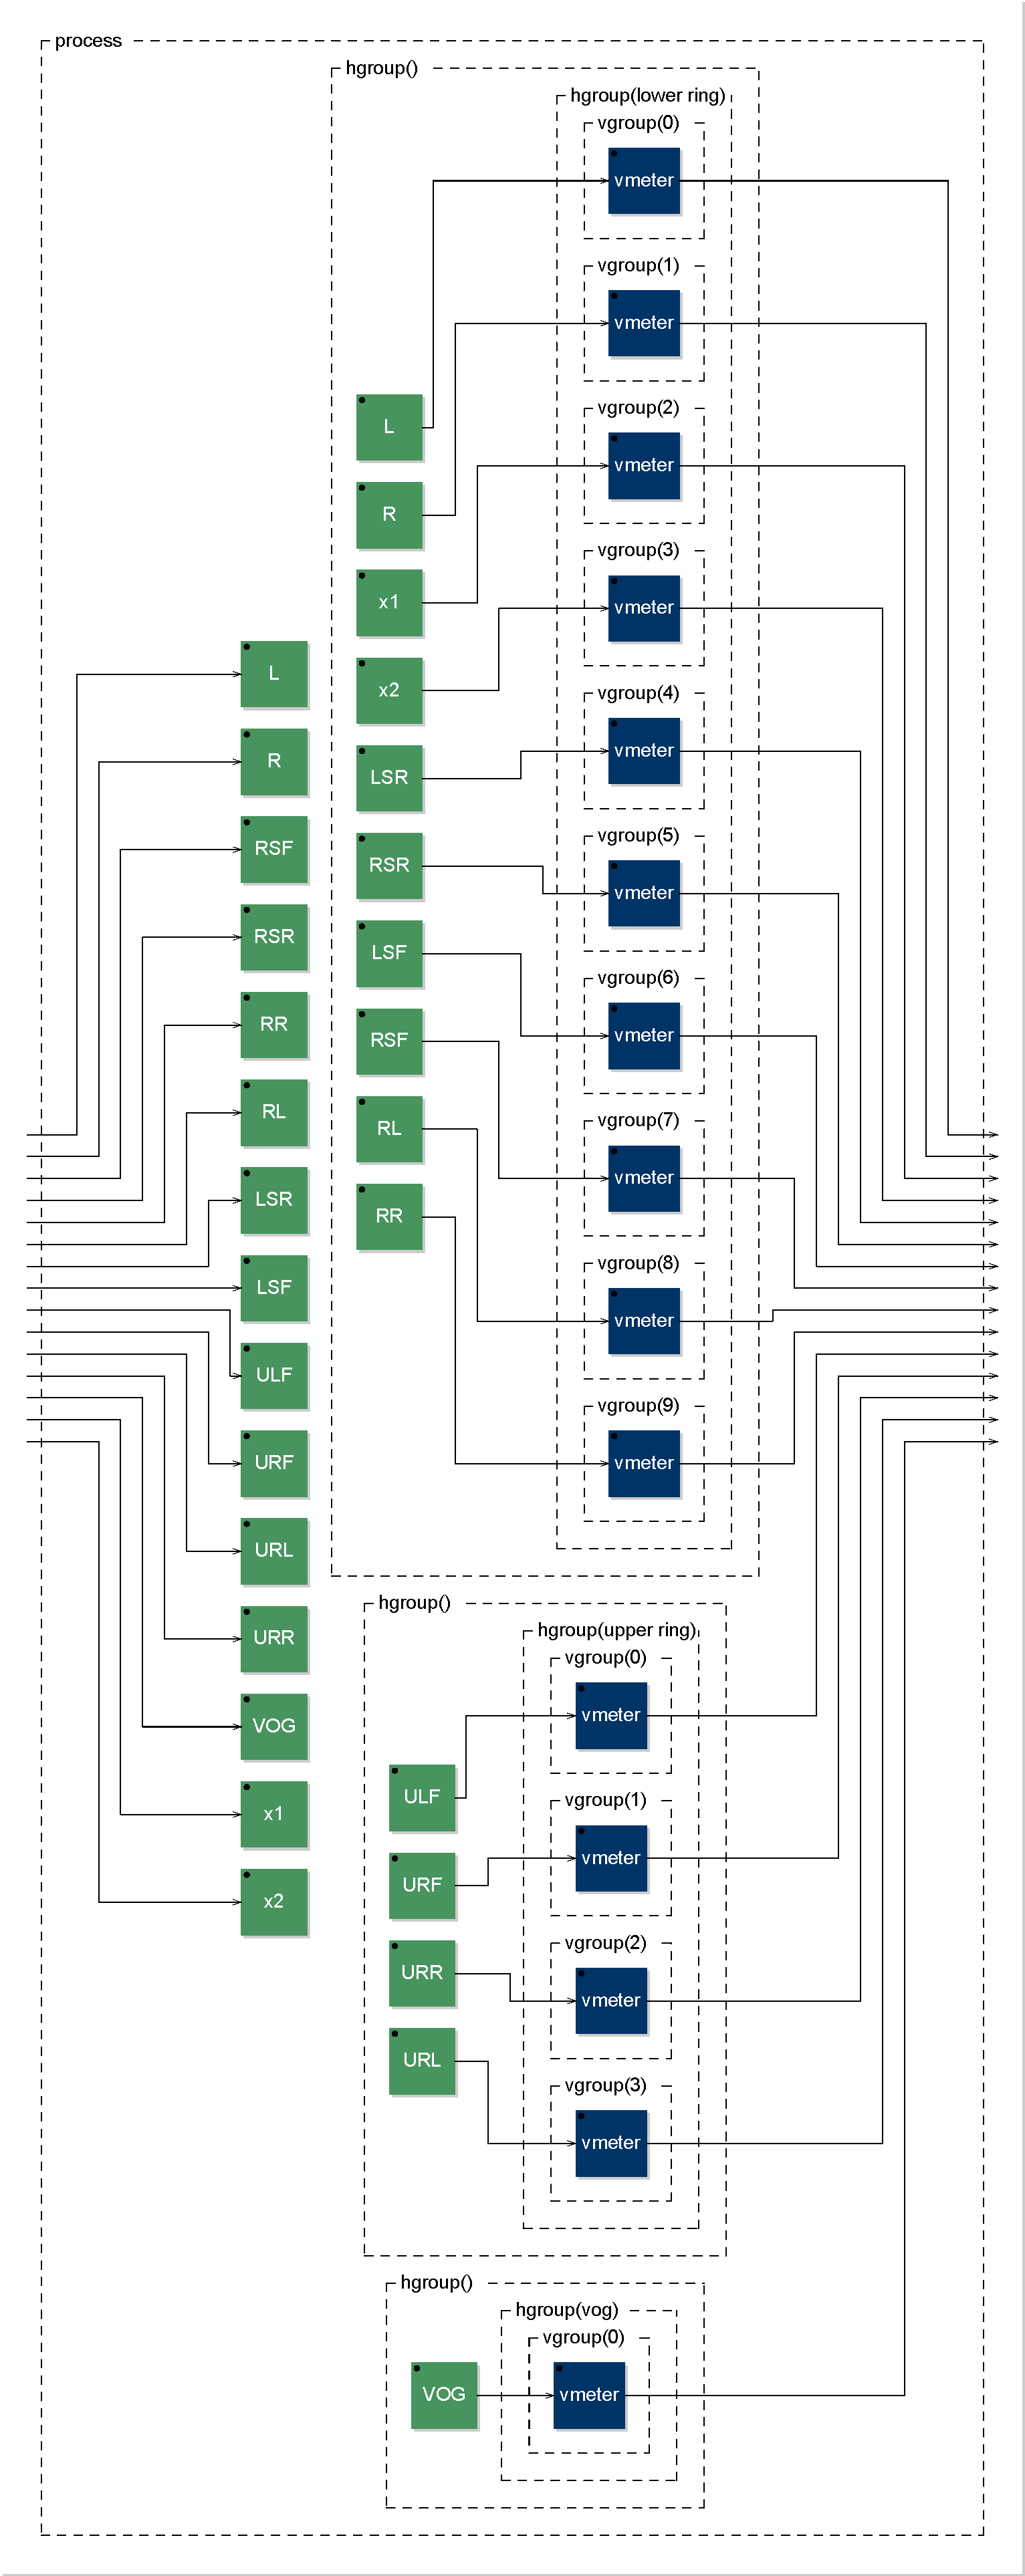
\includegraphics[width=\textwidth]{../svg/svg-01/process}
	\caption{Block diagram of \texttt{process}}
	\label{figure1}
\end{figure}

 \section{Notice} \label{notice}  
\begin{itemize}
	\item This document was generated using Faust version \faustversion\ on \faustdocdate.
	\item The value of a Faust program is the result of applying the signal transformer denoted by the expression to which the \texttt{process} identifier is bound to input signals, running at the $f_S$ sampling frequency.
	\item Faust (\emph{Functional Audio Stream}) is a functional programming language designed for synchronous real-time signal processing and synthesis applications. A Faust program is a set of bindings of identifiers to expressions that denote signal transformers. A signal $s$ in $S$ is a function mapping\footnote{Faust assumes that $\forall \, s \in S, \forall \, t \in \mathbb{Z}, s(t) = 0 \mathrm{\ when\ } t < 0$.} times $t \in \mathbb{Z}$ to values $s(t) \in \mathbb{R}$, while a signal transformer is a function from $S^n$ to $S^m$, where $n,m\in \mathbb{N}$. See the Faust manual for additional information (\textsf{http://faust.grame.fr}).
	\item Every mathematical formula derived from a Faust expression is assumed, in this document, to having been normalized (in an implementation-depen\-dent manner) by the Faust compiler.
	\item A block diagram is a graphical representation of the Faust binding of an identifier I to an expression E; each graph is put in a box labeled by I. Subexpressions of E are recursively displayed as long as the whole picture fits in one page.
	\item The \texttt{\faustdocdir/} directory may also include the following subdirectories:
\begin{itemize}
	\item	\texttt{cpp/} for Faust compiled code; 
	\item	\texttt{pdf/} which contains this document; 
	\item	\texttt{src/} for all Faust sources used (even libraries); 
	\item	\texttt{svg/} for block diagrams, encoded using the Scalable Vector Graphics format (\textsf{http://www.w3.org/Graphics/SVG/});
	\item	\texttt{tex/} for the \LaTeX\ source of this document.
\end{itemize}
\end{itemize}

 \section{Faust code listings} \label{listing}  This section provides the listings of the Faust code used to generate this document, including dependencies. 
\bigskip\bigskip
\begin{lstlisting}[caption=\texttt{KMH114\_channel\_map.dsp}]
declare name	"Channel mapping for Studio 114(C)";
declare version " 0.1 ";
declare author " Henrik Frisk " ;
declare license " BSD ";
declare copyright "(c) dinergy 2018 ";

//---------------`Channel mapping plugin` --------------------------
//
// Channel mapping plugin that takes 15 channels of input (center speaker included)
// and maps it to the channel/speaker configuration of the studio 114 according to:
//
// * 1 -> 1 (L)    
// * 2 -> 2 (R)    
// * 3 -> 5 (LSR)  
// * 4 -> 6 (RSR)  
// * 5 -> 7 (LSF)  
// * 6 -> 8 (RSF)  
// * 7 -> 9 (RL)   
// * 8 -> 10 (RR)  
// * 9 -> 11 (ULF) 
// * 10 -> 12 (URF) 
// * 11 -> 13 (URL) 
// * 12 -> 14 (URR) 		 
// * 13 -> 15 (VOG) 
// * 14 -> -        
//
//---------------------------------------------------

import("stdfaust.lib");

vmeter(x)	= attach(x, envelop(x) : vbargraph("[unit:dB]", -70, +5));
hmeter(x)	= attach(x, envelop(x) : hbargraph("[2][unit:dB]", -70, +5));
envelop         = abs : max ~ -(1.0/ma.SR) : max(ba.db2linear(-70)) : ba.linear2db;

process(L, R, RSF, RSR, RR, RL, LSR, LSF, ULF, URF, URL, URR, VOG, x1, x2) =
  hgroup("", (L, R, x1, x2, LSR, RSR, LSF, RSF, RL, RR) : hgroup("lower ring", par(i, 10, vgroup("%i", vmeter)))),
  hgroup("", (ULF, URF, URR, URL) : hgroup("upper ring", par(i, 4, vgroup("%i", vmeter)))),
  hgroup("", (VOG) : hgroup("vog", par(i, 1, vgroup("%i", vmeter))));
\end{lstlisting}


\bigskip\bigskip
\begin{lstlisting}[caption=\texttt{stdfaust.lib}]
//################################ stdfaust.lib ##########################################
// The purpose of this library is to give access to all the Faust standard libraries
// through a series of environment.
//########################################################################################

an = library("analyzers.lib");
ba = library("basics.lib");
co = library("compressors.lib");
de = library("delays.lib");
dm = library("demos.lib");
dx = library("dx7.lib");
en = library("envelopes.lib");
fi = library("filters.lib");
ho = library("hoa.lib");
ma = library("maths.lib");
ef = library("misceffects.lib");
os = library("oscillators.lib");
no = library("noises.lib");
pf = library("phaflangers.lib");
pm = library("physmodels.lib");
re = library("reverbs.lib");
ro = library("routes.lib");
sp = library("spats.lib");
si = library("signals.lib");
so = library("soundfiles.lib");
sy = library("synths.lib");
ve = library("vaeffects.lib");
sf = library("all.lib");
\end{lstlisting}


\bigskip\bigskip
\begin{lstlisting}[caption=\texttt{maths.lib}]
//################################### maths.lib ##########################################
//  Mathematic library for Faust. Its official prefix is `ma`.
//########################################################################################
// Some functions are implemented as Faust foreign functions of `math.h` functions
// that are not part of Faust's primitives. Defines also various constants and several
// utilities.
//########################################################################################

// ## History
// * 06/13/2016 [RM]	normalizing and integrating to new libraries
// * 07/08/2015	[YO]	documentation comments
// * 20/06/2014	[SL]	added FTZ function
// * 20/06/2014	[SL]	added FTZ function
// * 22/06/2013	[YO]	added float|double|quad variants of some foreign functions
// * 28/06/2005	[YO]	postfixed functions with 'f' to force float version instead of double
// * 28/06/2005	[YO]	removed 'modf' because it requires a pointer as argument

/************************************************************************
************************************************************************
FAUST library file
Copyright (C) 2003-2016 GRAME, Centre National de Creation Musicale
----------------------------------------------------------------------
This program is free software; you can redistribute it and/or modify
it under the terms of the GNU Lesser General Public License as
published by the Free Software Foundation; either version 2.1 of the
License, or (at your option) any later version.

This program is distributed in the hope that it will be useful,
but WITHOUT ANY WARRANTY; without even the implied warranty of
MERCHANTABILITY or FITNESS FOR A PARTICULAR PURPOSE.  See the
GNU Lesser General Public License for more details.

You should have received a copy of the GNU Lesser General Public
License along with the GNU C Library; if not, write to the Free
Software Foundation, Inc., 59 Temple Place, Suite 330, Boston, MA
02111-1307 USA.

EXCEPTION TO THE LGPL LICENSE : As a special exception, you may create a
larger FAUST program which directly or indirectly imports this library
file and still distribute the compiled code generated by the FAUST
compiler, or a modified version of this compiled code, under your own
copyright and license. This EXCEPTION TO THE LGPL LICENSE explicitly
grants you the right to freely choose the license for the resulting
compiled code. In particular the resulting compiled code has no obligation
to be LGPL or GPL. For example you are free to choose a commercial or
closed source license or any other license if you decide so.
************************************************************************
************************************************************************/

declare name "Faust Math Library";
declare version "2.1";
declare author "GRAME";
declare copyright "GRAME";
declare license "LGPL with exception";

//=============================Functions Reference========================================
//========================================================================================


//---------------------------------`(ma.)SR`---------------------------------------
// Current sampling rate (between 1000Hz and 192000Hz). Constant during
// program execution.
//
// #### Usage
//
// ```
// SR : _
// ```
//-----------------------------------------------------------------------------
SR 			= min(192000.0, max(1.0, fconstant(int fSamplingFreq, <math.h>)));


//---------------------------------`(ma.)BS`---------------------------------------
// Current block-size. Can change during the execution.
//
// #### Usage
//
// ```
// BS : _
// ```
//-----------------------------------------------------------------------------
BS          = fvariable(int count, <math.h>);


//---------------------------------`(ma.)PI`---------------------------------------
// Constant PI in double precision.
//
// #### Usage
//
// ```
// PI : _
// ```
//-----------------------------------------------------------------------------
PI          = 3.1415926535897932385;

//---------------------------------`(ma.)INFINITY`------------------------------
// Constant INFINITY inherited from `math.h`.
//
// #### Usage
//
// ```
// INFINITY : _
// ```
//-----------------------------------------------------------------------------
INFINITY = fconstant(float INFINITY, <math.h>);

//---------------------------------`(ma.)FTZ`---------------------------------------
// Flush to zero: force samples under the "maximum subnormal number"
// to be zero. Usually not needed in C++ because the architecture
// file take care of this, but can be useful in javascript for instance.
//
// #### Usage
//
// ```
// _ : ftz : _
// ```
//
// See : <http://docs.oracle.com/cd/E19957-01/806-3568/ncg_math.html>
//-----------------------------------------------------------------------------
FTZ(x)      = x * (abs(x) > 1.17549435e-38);


//---------------------------------`(ma.)neg`---------------------------------------
// Invert the sign (-x) of a signal.
//
// #### Usage
//
// ```
// _ : neg : _
// ```
//-----------------------------------------------------------------------------
neg(x)      = -x;


//-------`(ma.)sub(x,y)`------------------
// Subtract `x` and `y`.
//------------------------------
sub(x,y) = y-x;


//---------------------------------`(ma.)inv`---------------------------------------
// Compute the inverse (1/x) of the input signal.
//
// #### Usage
//
// ```
// _ : inv : _
// ```
//-----------------------------------------------------------------------------
inv(x)      = 1/x;


//---------------------------------`(ma.)cbrt`--------------------------------------
// Computes the cube root of of the input signal.
//
// #### Usage
//
// ```
// _ : cbrt : _
// ```
//-----------------------------------------------------------------------------
cbrt 		= ffunction(float cbrtf|cbrt|cbrtl (float), <math.h>,"");


//---------------------------------`(ma.)hypot`-------------------------------------
// Computes the euclidian distance of the two input signals
// sqrt(x*x+y*y) without undue overflow or underflow.
//
// #### Usage
//
// ```
// _,_ : hypot : _
// ```
//-----------------------------------------------------------------------------
hypot 		= ffunction(float hypotf|hypot|hypotl (float, float), <math.h>,"");


//---------------------------------`(ma.)ldexp`-------------------------------------
// Takes two input signals: x and n, and multiplies x by 2 to the power n.
//
// #### Usage
//
// ```
// _,_ : ldexp : _
// ```
//-----------------------------------------------------------------------------
ldexp 		= ffunction(float ldexpf|ldexp|ldexpl (float, int), <math.h>,"");


//---------------------------------`(ma.)scalb`-------------------------------------
// Takes two input signals: x and n, and multiplies x by 2 to the power n.
//
// #### Usage
//
// ```
// _,_ : scalb : _
// ```
//-----------------------------------------------------------------------------
scalb 		= ffunction(float scalbnf|scalbn|scalbnl (float, int), <math.h>,"");


//---------------------------------`(ma.)log1p`----------------------------------
// Computes log(1 + x) without undue loss of accuracy when x is nearly zero.
//
// #### Usage
//
// ```
// _ : log1p : _
// ```
//-----------------------------------------------------------------------------
log1p 		= ffunction(float log1pf|log1p|log1pl (float), <math.h>,"");


//---------------------------------`(ma.)logb`---------------------------------------
// Return exponent of the input signal as a floating-point number.
//
// #### Usage
//
// ```
// _ : logb : _
// ```
//-----------------------------------------------------------------------------
logb 		= ffunction(float logbf|logb|logbl (float), <math.h>,"");


//---------------------------------`(ma.)ilogb`-------------------------------------
// Return exponent of the input signal as an integer number.
//
// #### Usage
//
// ```
// _ : ilogb : _
// ```
//-----------------------------------------------------------------------------
ilogb 		= ffunction(int ilogbf|ilogb|ilogbl (float), <math.h>,"");


//---------------------------------`(ma.)log2`-------------------------------------
// Returns the base 2 logarithm of x.
//
// #### Usage
//
// ```
// _ : log2 : _
// ```
//-----------------------------------------------------------------------------
log2(x) = log(x)/log(2.0);


//---------------------------------`(ma.)expm1`-------------------------------------
// Return exponent of the input signal minus 1 with better precision.
//
// #### Usage
//
// ```
// _ : expm1 : _
// ```
//-----------------------------------------------------------------------------
expm1 		= ffunction(float expm1f|expm1|expm1l (float), <math.h>,"");


//---------------------------------`(ma.)acosh`-------------------------------------
// Computes the principle value of the inverse hyperbolic cosine
// of the input signal.
//
// #### Usage
//
// ```
// _ : acosh : _
// ```
//-----------------------------------------------------------------------------
acosh		= ffunction(float acoshf|acosh|acoshl (float), <math.h>, "");


//--------------------------------`(ma.)asinh`-----------------------------------
// Computes the inverse hyperbolic sine of the input signal.
//
// #### Usage
//
// ```
// _ : asinh : _
// ```
//-----------------------------------------------------------------------------
asinh		= ffunction(float asinhf|asinh|asinhl (float), <math.h>, "");


//--------------------------------`(ma.)atanh`-----------------------------------
// Computes the inverse hyperbolic tangent of the input signal.
//
// #### Usage
//
// ```
// _ : atanh : _
// ```
//-----------------------------------------------------------------------------
atanh		= ffunction(float atanhf|atanh|atanhl (float), <math.h>, "");


//---------------------------------`(ma.)sinh`---------------------------------------
// Computes the hyperbolic sine of the input signal.
//
// #### Usage
//
// ```
// _ : sinh : _
// ```
//-----------------------------------------------------------------------------
sinh		= ffunction(float sinhf|sinh|sinhl (float), <math.h>, "");


//---------------------------------`(ma.)cosh`--------------------------------------
// Computes the hyperbolic cosine of the input signal.
//
// #### Usage
//
// ```
// _ : cosh : _
// ```
//-----------------------------------------------------------------------------
cosh		= ffunction(float coshf|cosh|coshl (float), <math.h>, "");


//---------------------------------`(ma.)tanh`--------------------------------------
// Computes the hyperbolic tangent of the input signal.
//
// #### Usage
//
// ```
// _ : tanh : _
// ```
//-----------------------------------------------------------------------------
tanh		= ffunction(float tanhf|tanh|tanhl (float), <math.h>,"");


//---------------------------------`(ma.)erf`---------------------------------------
// Computes the error function of the input signal.
//
// #### Usage
//
// ```
// _ : erf : _
// ```
//-----------------------------------------------------------------------------
erf			= ffunction(float erff|erf|erfl(float), <math.h>,"");


//---------------------------------`(ma.)erfc`---------------------------------------
// Computes the complementary error function of the input signal.
//
// #### Usage
//
// ```
// _ : erfc : _
// ```
//-----------------------------------------------------------------------------
erfc		= ffunction(float erfcf|erfc|erfcl(float), <math.h>,"");


//---------------------------------`(ma.)gamma`-------------------------------------
// Computes the gamma function of the input signal.
//
// #### Usage
//
// ```
// _ : gamma : _
// ```
//-----------------------------------------------------------------------------
gamma		= ffunction(float tgammaf|tgamma|tgammal(float), <math.h>,"");


//---------------------------------`(ma.)lgamma`------------------------------------
// Calculates the natural logorithm of the absolute value of
// the gamma function of the input signal.
//
// #### Usage
//
// ```
// _ : lgamma : _
// ```
//-----------------------------------------------------------------------------
lgamma		= ffunction(float lgammaf|lgamma|lgammal(float), <math.h>,"");


//----------------------------------`(ma.)J0`---------------------------------------
// Computes the Bessel function of the first kind of order 0
// of the input signal.
//
// #### Usage
//
// ```
// _ : J0 : _
// ```
//-----------------------------------------------------------------------------
J0			= ffunction(float j0(float), <math.h>,"");


//----------------------------------`(ma.)J1`---------------------------------------
// Computes the Bessel function of the first kind of order 1
// of the input signal.
//
// #### Usage
//
// ```
// _ : J1 : _
// ```
//-----------------------------------------------------------------------------
J1			= ffunction(float j1(float), <math.h>,"");


//----------------------------------`(ma.)Jn`---------------------------------------
// Computes the Bessel function of the first kind of order n
// (first input signal) of the second input signal.
//
// #### Usage
//
// ```
// _,_ : Jn : _
// ```
//-----------------------------------------------------------------------------
Jn			= ffunction(float jn(int, float), <math.h>,"");


//----------------------------------`(ma.)Y0`---------------------------------------
// Computes the linearly independent Bessel function of the second kind
// of order 0 of the input signal.
//
// #### Usage
//
// ```
// _ : Y0 : _
// ```
//-----------------------------------------------------------------------------
Y0			= ffunction(float y0(float), <math.h>,"");


//----------------------------------`(ma.)Y1`---------------------------------------
// Computes the linearly independent Bessel function of the second kind
// of order 1 of the input signal.
//
// #### Usage
//
// ```
// _ : Y0 : _
// ```
//-----------------------------------------------------------------------------
Y1			= ffunction(float y1(float), <math.h>,"");


//----------------------------------`(ma.)Yn`---------------------------------------
// Computes the linearly independent Bessel function of the second kind
// of order n (first input signal) of the second input signal.
//
// #### Usage
//
// ```
// _,_ : Yn : _
// ```
//-----------------------------------------------------------------------------
Yn			= ffunction(float yn(int, float), <math.h>,"");


//----------------------------`(ma.)fabs`, `(ma.)fmax`, `(ma.)fmin`---------------------------
// Just for compatibility...
//
// ```
// fabs = abs
// fmax = max
// fmin = min
// ```
//-----------------------------------------------------------------------------
fabs = abs;
fmax = max;
fmin = min;

//-------------------------------`(ma.)np2`--------------------------------------
// Gives the next power of 2 of x.
//
// #### Usage
//
// ```
// np2(n) : _
// ```
//
// Where:
//
// * `n`: an integer
//-----------------------------------------------------------------------------
np2 = -(1) <: >>(1)|_ <: >>(2)|_ <: >>(4)|_ <: >>(8)|_ <: >>(16)|_ : +(1);


//-----------------------------`(ma.)frac`---------------------------------------
// Gives the fractional part of n.
//
// #### Usage
//
// ```
// frac(n) : _
// ```
//
// Where:
//
// * `n`: a decimal number
//------------------------------------------------------------------------------
frac(n) = n - floor(n);
decimal = frac;
// NOTE: decimal does the same thing as frac but using floor instead. JOS uses frac a lot
// in filters.lib so we decided to keep that one... decimal is declared though for
// backward compatibility.
// decimal(n)	= n - floor(n);

//-------------------------------`(ma.)modulo`---------------------------------------
// Modulus operation.
//
// #### Usage
//
// ```
// modulo(x,N) : _
// ```
//
// Where:
//
// * `x`: the numerator
// * `N`: the denominator
//------------------------------------------------------------------------------
modulo(x,N) = (x % N + N) % N;


//---------------`(ma.)isnan`----------------
// Return non-zero if and only if x is a NaN.
//
// #### Usage
//
// ```
// isnan(x)
// _ : isnan : _
// ```
//
// Where:
//
// * `x`: signal to analyse
//------------------------------------------
isnan 		= ffunction(int isnan (float),<math.h>,"");
nextafter	= ffunction(float nextafter(float, float),<math.h>,"");


//---------------------------`(ma.)chebychev`-------------------------------
// Chebychev transformation of order n.
//
// #### Usage
//
// ```
// _ : chebychev(n) : _
// ```
//
// Where:
//
// * `n`: the order of the polynomial
//
// #### Semantics
//
// ```
// T[0](x) = 1,
// T[1](x) = x,
// T[n](x) = 2x*T[n-1](x) - T[n-2](x)
// ```
//
// #### Reference
//
// <http://en.wikipedia.org/wiki/Chebyshev_polynomial>
//-------------------------------------------------------------------------
chebychev(0) = !:1;
chebychev(1) = _;
chebychev(n) = _ <: *(2)*chebychev(n-1)-chebychev(n-2);



//------------------------`(ma.)chebychevpoly`-------------------------------
// Linear combination of the first Chebyshev polynomials.
//
// #### Usage
//
// ```
// _ : chebychevpoly((c0,c1,...,cn)) : _
// ```
//
// Where:
//
// * `cn`: the different Chebychevs polynomials such that:
// 	chebychevpoly((c0,c1,...,cn)) = Sum of chebychev(i)*ci
//
// #### Reference
//
// <http://www.csounds.com/manual/html/chebyshevpoly.html>
//-------------------------------------------------------------------------
chebychevpoly(lcoef) = _ <: L(0,lcoef) :> _
	with {
		L(n,(c,cs)) = chebychev(n)*c, L(n+1,cs);
		L(n,c)      = chebychev(n)*c;
	};


//------------------`(ma.)diffn`----------------------------
// Negated first-order difference.
//
// #### Usage
//
// ```
// _ : diffn : _
// ```
//--------------------------------------------------------
diffn(x) = x' - x; // negated first-order difference

//------------------`(ma.)signum`----------------------------
// The signum function signum(x) is defined as
// -1 for x<0, 0 for x==0, and 1 for x>0;
//
// #### Usage
//
// ```
// _ : signum : _
// ```
//--------------------------------------------------------
signum(x) = (x>0)-(x<0);
\end{lstlisting}


\bigskip\bigskip
\begin{lstlisting}[caption=\texttt{basics.lib}]
//#################################### basics.lib ########################################
// A library of basic elements. Its official prefix is `ba`.
//########################################################################################
// A library of basic elements for Faust organized in 5 sections:
//
// * Conversion Tools
// * Counters and Time/Tempo Tools
// * Array Processing/Pattern Matching
// * Selectors (Conditions)
// * Other Tools (Misc)

//########################################################################################

/************************************************************************
************************************************************************
FAUST library file, GRAME section

Except where noted otherwise, Copyright (C) 2003-2017 by GRAME,
Centre National de Creation Musicale.
----------------------------------------------------------------------
GRAME LICENSE

This program is free software; you can redistribute it and/or modify
it under the terms of the GNU Lesser General Public License as
published by the Free Software Foundation; either version 2.1 of the
License, or (at your option) any later version.

This program is distributed in the hope that it will be useful,
but WITHOUT ANY WARRANTY; without even the implied warranty of
MERCHANTABILITY or FITNESS FOR A PARTICULAR PURPOSE.  See the
GNU Lesser General Public License for more details.

You should have received a copy of the GNU Lesser General Public
License along with the GNU C Library; if not, write to the Free
Software Foundation, Inc., 59 Temple Place, Suite 330, Boston, MA
02111-1307 USA.

EXCEPTION TO THE LGPL LICENSE : As a special exception, you may create a
larger FAUST program which directly or indirectly imports this library
file and still distribute the compiled code generated by the FAUST
compiler, or a modified version of this compiled code, under your own
copyright and license. This EXCEPTION TO THE LGPL LICENSE explicitly
grants you the right to freely choose the license for the resulting
compiled code. In particular the resulting compiled code has no obligation
to be LGPL or GPL. For example you are free to choose a commercial or
closed source license or any other license if you decide so.
************************************************************************
************************************************************************/

ma = library("maths.lib");
ro = library("routes.lib");
ba = library("basics.lib"); // so functions here can be copy/pasted out

declare name "Faust Basic Element Library";
declare version "0.0";

//=============================Conversion Tools===========================================
//========================================================================================


//-------`(ba.)samp2sec`----------
// Converts a number of samples to a duration in seconds.
// `samp2sec` is a standard Faust function.
//
// #### Usage
//
// ```
// samp2sec(n) : _
// ```
//
// Where:
//
// * `n`: number of samples
//----------------------------
samp2sec = /(ma.SR);


//-------`(ba.)sec2samp`----------
// Converts a duration in seconds to a number of samples.
// `samp2sec` is a standard Faust function.
//
// #### Usage
//
// ```
// sec2samp(d) : _
// ```
//
// Where:
//
// * `d`: duration in seconds
//----------------------------
sec2samp = *(ma.SR);


//-------`(ba.)db2linear`----------
// Converts a loudness in dB to a linear gain (0-1).
// `db2linear` is a standard Faust function.
//
// #### Usage
//
// ```
// db2linear(l) : _
// ```
//
// Where:
//
// * `l`: loudness in dB
//-----------------------------
db2linear(n) = pow(10, n/20.0);


//-------`(ba.)linear2db`----------
// Converts a linear gain (0-1) to a loudness in dB.
// `linear2db` is a standard Faust function.
//
// #### Usage
//
// ```
// linear2db(g) : _
// ```
//
// Where:
//
// * `g`: a linear gain
//-----------------------------
linear2db(n) = 20*log10(n);


//----------`(ba.)lin2LogGain`------------------
// Converts a linear gain (0-1) to a log gain (0-1).
//
// #### Usage
//
// ```
// _ : lin2LogGain : _
// ```
//---------------------------------------------
lin2LogGain = _ <: _*_;


//----------`(ba.)log2LinGain`------------------
// Converts a log gain (0-1) to a linear gain (0-1).
//
// #### Usage
//
// ```
// _ : log2LinGain : _
// ```
//---------------------------------------------
log2LinGain = sqrt;

// end GRAME section
//########################################################################################
/************************************************************************
FAUST library file, jos section

Except where noted otherwise, The Faust functions below in this
section are Copyright (C) 2003-2017 by Julius O. Smith III <jos@ccrma.stanford.edu>
([jos](http://ccrma.stanford.edu/~jos/)), and released under the
(MIT-style) [STK-4.3](#stk-4.3-license) license.

The MarkDown comments in this section are Copyright 2016-2017 by Romain
Michon and Julius O. Smith III, and are released under the
[CCA4I](https://creativecommons.org/licenses/by/4.0/) license (TODO: if/when Romain agrees)

************************************************************************/

//-------`(ba.)tau2pole`----------
// Returns a real pole giving exponential decay.
// Note that t60 (time to decay 60 dB) is ~6.91 time constants.
// `tau2pole` is a standard Faust function.
//
// #### Usage
//
// ```
// _ : smooth(tau2pole(tau)) : _
// ```
//
// Where:
//
// * `tau`: time-constant in seconds
//-----------------------------
  tau2pole(tau) = exp(-1.0/(tau*ma.SR));


//-------`(ba.)pole2tau`----------
// Returns the time-constant, in seconds, corresponding to the given real,
// positive pole in (0,1).
// `pole2tau` is a standard Faust function.
//
// #### Usage
//
// ```
// pole2tau(pole) : _
// ```
//
// Where:
//
// * `pole`: the pole
//-----------------------------
  pole2tau(pole) = -1.0/(log(pole)*ma.SR);


//-------`(ba.)midikey2hz`----------
// Converts a MIDI key number to a frequency in Hz (MIDI key 69 = A440).
// `midikey2hz` is a standard Faust function.
//
// #### Usage
//
// ```
// midikey2hz(mk) : _
// ```
//
// Where:
//
// * `mk`: the MIDI key number
//-----------------------------
  midikey2hz(mk)  = 440.0*pow(2.0, (mk-69.0)/12);


//-------`(ba.)hz2midikey`----------
// Converts a frequency in Hz to a MIDI key number (MIDI key 69 = A440).
// `hz2midikey` is a standard Faust function.
//
// #### Usage
//
// ```
// hz2midikey(f) : _
// ```
//
// Where:
//
// * `f`: frequency in Hz
//-----------------------------
  hz2midikey(f) = 12*ma.log2(f/440.0) + 69.0;


//-------`(ba.)pianokey2hz`----------
// Converts a piano key number to a frequency in Hz (piano key 49 = A440).
//
// #### Usage
//
// ```
// pianokey2hz(pk) : _
// ```
//
// Where:
//
// * `pk`: the piano key number
//-----------------------------
  pianokey2hz(pk) = 440.0*pow(2.0, (pk-49.0)/12);


//-------`(ba.)hz2pianokey`----------
// Converts a frequency in Hz to a piano key number (piano key 49 = A440).
//
// #### Usage
//
// ```
// hz2pianokey(f) : _
// ```
//
// Where:
//
// * `f`: frequency in Hz
//-----------------------------
  hz2pianokey(f)  = 12*ma.log2(f/440.0) + 49.0;

// end jos section
//########################################################################################
/************************************************************************
FAUST library file, GRAME section 2
************************************************************************/

//==============================Counters and Time/Tempo Tools=============================
//========================================================================================

//----------------------------`(ba.)countdown`------------------------------
// Starts counting down from n included to 0. While trig is 1 the output is n.
// The countdown starts with the transition of trig from 1 to 0. At the end
// of the countdown the output value will remain at 0 until the next trig.
// `countdown` is a standard Faust function.
//
// #### Usage
//
// ```
// countdown(n,trig) : _
// ```
//
// Where:
//
// * `count`: the starting point of the countdown
// * `trig`: the trigger signal (1: start at `n`; 0: decrease until 0)
//-----------------------------------------------------------------------------
countdown(count, trig)	= \(c).(if(trig>0, count, max(0, c-1))) ~_;


//----------------------------`(ba.)countup`--------------------------------
// Starts counting up from 0 to n included. While trig is 1 the output is 0.
// The countup starts with the transition of trig from 1 to 0. At the end
// of the countup the output value will remain at n until the next trig.
// `countup` is a standard Faust function.
//
// #### Usage
//
// ```
// countup(n,trig) : _
// ```
//
// Where:
//
// * `count`: the maximum count value
// * `trig`: the trigger signal (1: start at 0; 0: increase until `n`)
//-----------------------------------------------------------------------------
countup(count, trig)	= \(c).(if(trig>0, 0, min(count, c+1))) ~_;


//--------------------`(ba.)sweep`--------------------------
// Counts from 0 to `period` samples repeatedly, while `run` is 1.
// Outsputs zero while `run` is 0.
//
// #### Usage
//
// ```
// sweep(period,run) : _
// ```
//-----------------------------------------------------------------
// Author: Jonatan Liljedahl, markdown by RM
sweep = %(int(*:max(1)))~+(1);


//-------`(ba.)time`----------
// A simple timer that counts every samples from the beginning of the process.
// `time` is a standard Faust function.
//
// #### Usage
//
// ```
// time : _
// ```
//------------------------
time = (+(1)~_ ) - 1;


//-------`(ba.)tempo`----------
// Converts a tempo in BPM into a number of samples.
//
// #### Usage
//
// ```
// tempo(t) : _
// ```
//
// Where:
//
// * `t`: tempo in BPM
//------------------------
tempo(t) = (60*ma.SR)/t;


//-------`(ba.)period`----------
// Basic sawtooth wave of period `p`.
//
// #### Usage
//
// ```
// period(p) : _
// ```
//
// Where:
//
// * `p`: period as a number of samples
//------------------------
// NOTE: may be this should go in oscillators.lib
period(p) = %(int(p))~+(1');


//-------`(ba.)pulse`----------
// Pulses (10000) generated at period `p`.
//
// #### Usage
//
// ```
// pulse(p) : _
// ```
//
// Where:
//
// * `p`: period as a number of samples
//------------------------
// NOTE: may be this should go in oscillators.lib
pulse(p) = period(p)==0;


//-------`(ba.)pulsen`----------
// Pulses (11110000) of length `n` generated at period `p`.
//
// #### Usage
//
// ```
// pulsen(n,p) : _
// ```
//
// Where:
//
// * `n`: the length of the pulse as a number of samples
// * `p`: period as a number of samples
//------------------------
// NOTE: may be this should go in oscillators.lib
pulsen(n,p) = period(p)<n;


//-----------------------`(ba.)cycle`---------------------------
// Split nonzero input values into `n` cycles.
//
// #### Usage
//
// ```
// _ : cycle(n) <:
// ```
//
// Where:
//
// * `n`: the number of cycles/output signals
//---------------------------------------------------------
// Author: Mike Olsen
cycle(n) = _ <: par(i,n,resetCtr(n,(i+1)));


//-------`(ba.)beat`----------
// Pulses at tempo `t`.
// `beat` is a standard Faust function.
//
// #### Usage
//
// ```
// beat(t) : _
// ```
//
// Where:
//
// * `t`: tempo in BPM
//------------------------
beat(t) = pulse(tempo(t));


//----------------------------`(ba.)pulse_countup`-----------------------------------
// Starts counting up pulses. While trig is 1 the output is
// counting up, while trig is 0 the counter is reset to 0.
//
// #### Usage
//
// ```
// _ : pulse_countup(trig) : _
// ```
//
// Where:
//
// * `trig`: the trigger signal (1: start at next pulse; 0: reset to 0)
//------------------------------------------------------------------------------
//TODO: author "Vince"
pulse_countup(t) =  + ~ _ * t ;


//----------------------------`(ba.)pulse_countdown`---------------------------------
// Starts counting down pulses. While trig is 1 the output is
// counting down, while trig is 0 the counter is reset to 0.
//
// #### Usage
//
// ```
// _ : pulse_countdown(trig) : _
// ```
//
// Where:
//
// * `trig`: the trigger signal (1: start at next pulse; 0: reset to 0)
//------------------------------------------------------------------------------
//TODO: author "Vince"
pulse_countdown(t) =  - ~ _ * t ;


//----------------------------`(ba.)pulse_countup_loop`------------------------------
// Starts counting up pulses from 0 to n included. While trig is 1 the output is
// counting up, while trig is 0 the counter is reset to 0. At the end
// of the countup (n) the output value will be reset to 0.
//
// #### Usage
//
// ```
// _ : pulse_countup_loop(n,trig) : _
// ```
//
// Where:
//
// * `n`: the highest number of the countup (included) before reset to 0.
// * `trig`: the trigger signal (1: start at next pulse; 0: reset to 0)
//------------------------------------------------------------------------------
//TODO: author "Vince"
pulse_countup_loop(n, t) =  + ~ cond(n)*t
with {
  cond(n) =  _ <: _ * (_ <= n) ;
};


//-----------------------`(ba.)resetCtr`------------------------
// Function that lets through the mth impulse out of
// each consecutive group of `n` impulses.
//
// #### Usage
//
// ```
// _ : resetCtr(n,m) : _
// ```
//
// Where:
//
// * `n`: the total number of impulses being split
// * `m`: index of impulse to allow to be output
//---------------------------------------------------------
// Author: Mike Olsen
resetCtr(n,m) = _ <: (_,pulse_countup_loop(n-1,1)) : (_,(_==m)) : *;


//----------------------------`(ba.)pulse_countdown_loop`----------------------------
// Starts counting down pulses from 0 to n included. While trig is 1 the output
// is counting down, while trig is 0 the counter is reset to 0. At the end
// of the countdown (n) the output value will be reset to 0.
//
// #### Usage
//
// ```
// _ : pulse_coundown_loop(n,trig) : _
// ```
//
// Where:
//
// * `n`: the highest number of the countup (included) before reset to 0.
// * `trig`: the trigger signal (1: start at next pulse; 0: reset to 0)
//------------------------------------------------------------------------------
//TODO: author "Vince:
pulse_countdown_loop(n, t) =  - ~ cond(n)*t
with {
  cond(n) =  _ <: _ * (_ >= n) ;
};



//===============================Array Processing/Pattern Matching========================
//========================================================================================

//---------------------------------`(ba.)count`---------------------------------
// Count the number of elements of list l.
// `count` is a standard Faust function.
//
// #### Usage
//
// ```
// count(l)
// count ((10,20,30,40)) -> 4
// ```
//
// Where:
//
// * `l`: list of elements
//-----------------------------------------------------------------------------
count ((xs, xxs)) = 1 + count(xxs);
count (xx) = 1;


//-------------------------------`(ba.)take`-----------------------------------
// Take an element from a list.
// `take` is a standard Faust function.
//
// #### Usage
//
// ```
// take(e,l)
// take(3,(10,20,30,40)) -> 30
// ```
//
// Where:
//
// * `p`: position (starting at 1)
// * `l`: list of elements
//-----------------------------------------------------------------------------
take (1, (xs, xxs)) 	= xs;
take (1, xs) 			= xs;
take (nn, (xs, xxs)) 	= take (nn-1, xxs);


//----------------------------`(ba.)subseq`--------------------------------
// Extract a part of a list.
//
// #### Usage
//
// ```
// subseq(l, p, n)
// subseq((10,20,30,40,50,60), 1, 3) -> (20,30,40)
// subseq((10,20,30,40,50,60), 4, 1) -> 50
// ```
//
// Where:
//
// * `l`: list
// * `p`: start point (0: begin of list)
// * `n`: number of elements
//
// #### Note:
//
// Faust doesn't have proper lists. Lists are simulated with parallel
// compositions and there is no empty list
//-----------------------------------------------------------------------------
subseq((head, tail), 0, 1)      = head;
subseq((head, tail), 0, n)      = head, subseq(tail, 0, n-1);
subseq((head, tail), p, n)      = subseq(tail, p-1, n);
subseq(head, 0, n)              = head;


//============================Selectors (Conditions)======================================
//========================================================================================

//-----------------------------`(ba.)if`-----------------------------------
// if-then-else implemented with a select2.
//
// #### Usage
//
// *   `if(c, t, e) : _`
//
// Where:
//
// * `c`: condition
// * `t`: signal selected while c is true
// * `e`: signal selected while c is false
//-----------------------------------------------------------------------------
if(cond,thn,els) = select2(cond,els,thn);
// TODO: perhaps it would make more sense to have an if(a,b) and an ifelse(a,b,c)?

//-----------------------------`(ba.)selector`---------------------------------
// Selects the ith input among n at compile time.
//
// #### Usage
//
// ```
// selector(i,n)
// _,_,_,_ : selector(2,4) : _  // selects the 3rd input among 4
// ```
//
// Where:
//
// * `i`: input to select (`int`, numbered from 0, known at compile time)
// * `n`: number of inputs (`int`, known at compile time, `n > i`)
//
// There is also cselector for selecting among complex input signals of the form (real,imag).
//
//-----------------------------------------------------------------------------
selector(i,n) = par(j, n, S(i, j))    with { S(i,i) = _; S(i,j) = !; };
cselector(i,n) = par(j, n, S(i, j))    with { S(i,i) = (_,_); S(i,j) = (!,!); }; // for complex numbers


//-----------------------------`(ba.)selectn`---------------------------------
// Selects the ith input among N at run time.
//
// #### Usage
//
// ```
// selectn(N,i)
// _,_,_,_ : selectn(4,2) : _  // selects the 3rd input among 4
// ```
//
// Where:
//
// * `N`: number of inputs (int, known at compile time, N > 0)
// * `i`: input to select (int, numbered from 0)
//
// #### Example test program
//
// ```
// N=64;
// process = par(n,N, (par(i,N,i) : selectn(N,n)));
// ```
//-----------------------------------------------------------------------------
selectn(N,i) = S(N,0)
    with {
       S(1,offset) = _;
       S(n,offset) = S(left, offset), S(right, offset+left) : select2(i >= offset+left)
            with {
                right = int(n/2);
                left  = n-right;
            };
    };


//--------------------`(ba.)select2stereo`--------------------
// Select between 2 stereo signals.
//
// #### Usage
//
// ```
// _,_,_,_ : select2stereo(bpc) : _,_,_,_
// ```
//
// Where:
//
// * `bpc`: the selector switch (0/1)
//------------------------------------------------------------
  select2stereo(bpc) = ro.cross2 : select2(bpc), select2(bpc) : _,_;
//=====================================Other==============================================
//========================================================================================

//----------------------------`(ba.)latch`--------------------------------
// Latch input on positive-going transition of "clock" ("sample-and-hold").
//
// #### Usage
//
// ```
// _ : latch(clocksig) : _
// ```
//
// Where:
//
// * `clocksig`: hold trigger (0 for hold, 1 for bypass)
//------------------------------------------------------------
  latch(c,x) = x * s : + ~ *(1-s) with { s = ((c'<=0)&(c>0)); };


//--------------------------`(ba.)sAndH`-------------------------------
// Sample And Hold.
// `sAndH` is a standard Faust function.
//
// #### Usage
//
// ```
// _ : sAndH(t) : _
// ```
//
// Where:
//
// * `t`: hold trigger (0 for hold, 1 for bypass)
//----------------------------------------------------------------
// Author: RM
sAndH(t) = select2(t,_,_)~_;


//--------------------------`(ba.)downSample`-------------------------------
// Down sample a signal. WARNING: this function doesn't change the
// rate of a signal, it just holds samples...
// `downSample` is a standard Faust function.
//
// #### Usage
//
// ```
// _ : downSample(freq) : _
// ```
//
// Where:
//
// * `freq`: new rate in Hz
//----------------------------------------------------------------
// Author: RM
downSample(freq) = sAndH(hold)
with{
  hold = time%int(ma.SR/freq) == 0;
};


//------------------`(ba.)peakhold`---------------------------
// Outputs current max value above zero.
//
// #### Usage
//
// ```
// _ : peakhold(mode) : _;
// ```
//
// Where:
//
// `mode` means: 0 - Pass through. A single sample 0 trigger will work as a reset.
//    1 - Track and hold max value.
//----------------------------------------------------------------
// TODO: author Jonatan Liljedahl, revised by RM
peakhold = (*,_:max) ~ _;


//------------------`(ba.)peakholder`---------------------------
// Tracks abs peak and holds peak for 'holdtime' samples.
//
// #### Usage
//
// ```
// _ : peakholder(holdtime) : _;
// ```
//----------------------------------------------------------------
// TODO: author Jonatan Liljedahl
peakholder(holdtime) = peakhold2 ~ reset : (!,_) with {
    reset = ba.sweep(holdtime) > 0;
    // first out is gate that is 1 while holding last peak
    peakhold2 = _,abs <: peakhold,!,_ <: >=,_,!;
};


//--------------------------`(ba.)impulsify`---------------------------
// Turns the signal from a button into an impulse (1,0,0,... when
// button turns on).
// `impulsify` is a standard Faust function.
//
// #### Usage
//
// ```
// button("gate") : impulsify ;
// ```
//----------------------------------------------------------------
impulsify = _ <: _,mem : - : >(0);


//-----------------------`(ba.)automat`------------------------------
// Record and replay to the values the input signal in a loop.
//
// #### Usage
//
// ```
// hslider(...) : automat(bps, size, init) : _
// ```
//-----------------------------------------------------------------------
automat(bps, size, init, input) = rwtable(size+1, init, windex, input, rindex)
with {
	clock 	= beat(bps);
	rindex 	= int(clock) : (+ : %(size)) ~ _;		// each clock read the next entry of the table
	windex 	= if (timeToRenew, rindex, size);		// we ignore input unless it is time to renew
	timeToRenew 	= int(clock) & (inputHasMoved | (input <= init));
	inputHasMoved 	= abs(input-input') : countfrom(int(clock)') : >(0);
	countfrom(reset) = (+ : if(reset, 0, _)) ~ _;
};


//-----------------`(ba.)bpf`-------------------
// bpf is an environment (a group of related definitions) that can be used to
// create break-point functions. It contains three functions :
//
// * `start(x,y)` to start a break-point function
// * `end(x,y)` to end a break-point function
// * `point(x,y)` to add intermediate points to a break-point function
//
// A minimal break-point function must contain at least a start and an end point :
//
// ```
// f = bpf.start(x0,y0) : bpf.end(x1,y1);
// ```
//
// A more involved break-point function can contains any number of intermediate
// points:
//
// ```
// f = bpf.start(x0,y0) : bpf.point(x1,y1) : bpf.point(x2,y2) : bpf.end(x3,y3);
// ```
//
// In any case the `x_{i}` must be in increasing order (for all `i`, `x_{i} < x_{i+1}`).
// For example the following definition :
//
// ```
// f = bpf.start(x0,y0) : ... : bpf.point(xi,yi) : ... : bpf.end(xn,yn);
// ```
//
// implements a break-point function f such that :
//
// * `f(x) = y_{0}` when `x < x_{0}`
// * `f(x) = y_{n}` when `x > x_{n}`
// * `f(x) = y_{i} + (y_{i+1}-y_{i})*(x-x_{i})/(x_{i+1}-x_{i})` when `x_{i} <= x`
// and `x < x_{i+1}`
//
// `bpf` is a standard Faust function.
//--------------------------------------------------------
bpf = environment
{
  // Start a break-point function
  start(x0,y0) = \(x).(x0,y0,x,y0);
  // Add a break-point
  point(x1,y1) = \(x0,y0,x,y).(x1, y1, x , if (x < x0, y, if (x < x1, y0 + (x-x0)*(y1-y0)/(x1-x0), y1)));
  // End a break-point function
  end  (x1,y1) = \(x0,y0,x,y).(if (x < x0, y, if (x < x1, y0 + (x-x0)*(y1-y0)/(x1-x0), y1)));
};


//-------------------`(ba.)listInterp`-------------------------
// Linearly interpolates between the elements of a list.
//
// #### Usage
//
// ```
// foo = listInterp((800,400,350,450,325),index);
// i = 1.69; // range is 0-4
// process = foo(i);
// ```
//
// Where:
//
// * `index`: the index (float) to interpolate between the different values.
// The range of `index` depends on the size of the list.
//------------------------------------------------------------
// Author: RM
listInterp(v) =
  bpf.start(0,take(1,v)) :
  seq(i,count(v)-2,bpf.point(i+1,take(i+2,v))) :
  bpf.end(count(v)-1,take(count(v),v));


//-------------------`(ba.)bypass1`-------------------------
// Takes a mono input signal, route it to `e` and bypass it if `bpc = 1`.
// `bypass1` is a standard Faust function.
//
// #### Usage
//
// ```
// _ : bypass1(bpc,e) : _
// ```
//
// Where:
//
// * `bpc`: bypass switch (0/1)
// * `e`: a mono effect
//------------------------------------------------------------
// Author: JOS
// License: STK-4.3
bypass1(bpc,e) = _ <: select2(bpc,(inswitch:e),_)
  with {
    inswitch = select2(bpc,_,0);
  };

//-------------------`(ba.)bypass2`-------------------------
// Takes a stereo input signal, route it to `e` and bypass it if `bpc = 1`.
// `bypass2` is a standard Faust function.
//
// #### Usage
//
// ```
// _,_ : bypass2(bpc,e) : _,_
// ```
//
// Where:
//
// * `bpc`: bypass switch (0/1)
// * `e`: a stereo effect
//------------------------------------------------------------
// Author: JOS
// License: STK-4.3
bypass2(bpc,e) = _,_ <: ((inswitch:e),_,_) : select2stereo(bpc)
  with {
    inswitch = _,_ : (select2(bpc,_,0), select2(bpc,_,0)) : _,_;
  };

//-------------------`(ba.)bypass1to2`-------------------------
// Bypass switch for effect `e` having mono input signal and stereo output.
// Effect `e` is bypassed if `bpc = 1`.
// `bypass1to2` is a standard Faust function.
//
// #### Usage
//
// ```
// _ : bypass1(bpc,e) : _,_
// ```
//
// Where:
//
// * `bpc`: bypass switch (0/1)
// * `e`: a mono-to-stereo effect
//------------------------------------------------------------
// Author: JOS
// License: STK-4.3
bypass1to2(bpc,e) = _ <: ((inswitch:e),_,_) : ba.select2stereo(bpc)
  with {
    inswitch = select2(bpc,_,0);
  };

//----------------------------`(ba.)toggle`------------------------------------------
// Triggered by the change of 0 to 1, it toggles the output value
// between 0 and 1.
//
// #### Usage
//
// ```
// _ : toggle : _
// ```
// #### Examples
//
// ```
// button("toggle") : toggle : vbargraph("output", 0, 1)
// (an.amp_follower(0.1) > 0.01) : toggle : vbargraph("output", 0, 1) // takes audio input
// ```
//
//------------------------------------------------------------------------------
// TODO: author "Vince"
toggle = trig : loop
  with {
    trig(x) = (x-x') == 1;
    loop = (_ != _) ~ _ ;
  };


//----------------------------`(ba.)on_and_off`------------------------------------------
// The first channel set the output to 1, the second channel to 0.
//
// #### Usage
//
// ```
// _ , _ : on_and_off : _
// ```
//
// #### Example
//
// ```
// button("on"), button("off") : on_and_off : vbargraph("output", 0, 1)
// ```
//
//------------------------------------------------------------------------------
// TODO: author "Vince"
on_and_off(a, b) = (a : trig) : loop(b)
with {
  trig(x) = (x-x') == 1;
  loop(b) = + ~ (_ >= 1) * ((b : trig) == 0) ;
};


//-----------------------------`(ba.)selectoutn`---------------------------------
// Route input to the output among N at run time.
//
// #### Usage
//
// ```
// _ : selectoutn(n, s) : _,_,...n
// ```
//
// Where:
//
// * `n`: number of outputs (int, known at compile time, N > 0)
// * `s`: output number to route to (int, numbered from 0) (i.e. slider)
//
// #### Example
//
// ```
// process = 1 : selectoutn(3, sel) : par(i,3,bar) ;
// sel = hslider("volume",0,0,2,1) : int;
// bar = vbargraph("v.bargraph", 0, 1);
// ```
//--------------------------------------------------------------------------
// TODO: author "Vince"
selectoutn(n, s) = _ <: par(i,n, _* (s==i) ) ;

//=================================Sliding Reduce=========================================
// Provides various operations on the last N samples using a high order
// `slidingReduce(op,N,maxN,disabledVal,x)`` fold-like function :
//
// * `slidingSumN(n,maxn)`: the sliding sum of the last n input samples
// * `slidingMaxN(n,maxn)`: the sliding max of the last n input samples
// * `slidingMinN(n,maxn)`: the sliding min of the last n input samples
// * `slidingMeanN(n,maxn)`: the sliding mean of the last n input samples
// * `slidingRMSn(n,maxn)`: the sliding RMS of the last n input samples
//
// #### Working Principle
//
// If we want the maximum of the last 8 values, we can do that as:
//
// ```
// simpleMax(x) =
//  (
//    (
//      max(x@0,x@1),
//      max(x@2,x@3)
//    ) :max
//  ),
//  (
//    (
//      max(x@4,x@5),
//      max(x@6,x@7)
//    ) :max
//  )
//  :max;
// ```
//
// `max(x@2,x@3)` is the same as `max(x@0,x@1)@2` but the latter re-uses a
// value we already computed,so is more efficient. Using the same trick for
// values 4 trough 7, we can write:
//
// ```
// efficientMax(x)=
//  (
//    (
//      max(x@0,x@1),
//      max(x@0,x@1)@2
//    ) :max
//  ),
//  (
//    (
//      max(x@0,x@1),
//      max(x@0,x@1)@2
//    ) :max@4
//  )
//  :max;
// ```
//
// We can rewrite it recursively, so it becomes possible to get the maximum at
// have any number of values, as long as it's a power of 2.
//
// ```
// recursiveMax =
//  case {
//    (1,x) => x;
//    (N,x) =>  max(recursiveMax(N/2,x) , recursiveMax(N/2,x)@(N/2));
//  };
// ```
//
// What if we want to look at a number of values that's not a power of 2?
// For each value, we will have to decide whether to use it or not.
// If N is bigger than the index of the value, we use it, otherwise we replace
// it with (`0-(ma.INFINITY)`):
//
// ```
// variableMax(N,x) =
//  max(
//    max(
//      (
//        (x@0 : useVal(0)),
//        (x@1 : useVal(1))
//      ):max,
//      (
//        (x@2 : useVal(2)),
//        (x@3 : useVal(3))
//      ):max
//    ),
//    max(
//      (
//        (x@4 : useVal(4)),
//        (x@5 : useVal(5))
//      ):max,
//      (
//        (x@6 : useVal(6)),
//        (x@7 : useVal(7))
//      ):max
//    )
//  )
//  with{
//  useVal(i) = select2( (N>=i) , (0-(ma.INFINITY)),_);
// };
// ```
//
// Now it becomes impossible to re-use any values. To fix that let's first look
// at how we'd implement it using recursiveMax, but with a fixed N that is not
// a power of 2. For example, this is how you'd do it with `N=3`:
//
// ```
// binaryMaxThree(x) =
//  (
//    recursiveMax(1,x)@0, // the first x
//    recursiveMax(2,x)@1  // the second and third x
//  ):max;
// ```
//
// `N=6`
//
// ```
// binaryMaxSix(x) =
//  (
//    recursiveMax(2,x)@0, // first two
//    recursiveMax(4,x)@2  // third trough sixt
//  ):max;
// ```
//
// Note that `recursiveMax(2,x)` is used at a different delay then in
// `binaryMaxThree`, since it represents 1 and 2, not 2 and 3. Each block is
// delayed the combined size of the previous blocks.
//
// `N=7`
//
// ```
// binaryMaxSeven(x) =
//  (
//    (
//      recursiveMax(1,x)@0, // first x
//      recursiveMax(2,x)@1  // second and third
//    ):max,
//    (
//      recursiveMax(4,x)@3  // fourth trough seventh
//    )
//  ):max;
// ```
//
// To make a variable version, we need to know which powers of two are used,
// and at which delay time.
//
// Then it becomes a matter of:
//
// * lining up all the different block sizes in parallel:  the first `par()`
//  statement
// * delaying each the appropriate amount: `sumOfPrevBlockSizes()`
// * turning it on or off: `useVal()`
// * getting the maximum of all of them: `combine()`
//
// In faust, we can only do that for a fixed maximum number of values: `maxN`
//
// ```
// variableBinaryMaxN(N,maxN,x) =
//  par(i,maxNrBits,recursiveMax(pow2(i),x)@sumOfPrevBlockSizes(N,maxN,i)  : useVal(i)) : combine(maxNrBits) with {
//    // The sum of all the sizes of the previous blocks
//    sumOfPrevBlockSizes(N,maxN,0) = 0;
//    sumOfPrevBlockSizes(N,maxN,i) = (ba.subseq((allBlockSizes(N,maxN)),0,i):>_);
//    allBlockSizes(N,maxN) = par(i, maxNrBits, pow2(i) * isUsed(i) );
//    maxNrBits = int2nrOfBits(maxN);
//    // get the maximum of all blocks
//    combine(2) = max;
//    combine(N) = max(combine(N-1),_);
//    // Decide wether or not to use a certain value, based on N
//    useVal(i) = select2( isUsed(i), (0-(ma.INFINITY)),_);
//    isUsed(i) = ba.take(i+1,(int2bin(N,maxN)));
//  };
// ```
//========================================================================================
// Section contributed by Bart Brouns (bart@magnetophon.nl).
// SPDX-License-Identifier: GPL-3.0
// Copyright (C) 2018 Bart Brouns

//-----------------------------`(ba.)slidingReduce`-----------------------------
// Fold-like high order function. Apply a commutative binary operation `<op>` to
// the last `<n>` consecutive samples of a signal `<x>`. For example :
// `slidingReduce(max,128,128,-(ma.INFINITY))` will compute the maximum of the last
// 128 samples. The output is updated each sample, unlike reduce, where the
// output is constant for the duration of a block
//
// #### Usage
//
// ```
// _ : slidingReduce(op,N,maxN,disabledVal) : _
// ```
//
// Where:
//
// * `N`: the number of values to process
// * `maxN`: the maximum number of values to process, needs to be a power of 2
// * `op`: the operator. Needs to be a commutative one.
// * `disabledVal`: the value to use when we want to ignore a value.
//
// In other words, `op(x,disabledVal)` should equal to `x`. For example,
// `+(x,0)` equals `x` and `min(x,ma.INFINITY)` equals `x`. So if we want to
// calculate the sum, we need to give 0 as `disabledVal`, and if we want the
// minimum, we need to give `ma.INFINITY` as `disabledVal`.
//------------------------------------------------------------------------------
slidingReduce(op,N,maxN,disabledVal,x) =
  par(i,maxNrBits,fixedDelayOp(pow2(i),x)@sumOfPrevBlockSizes(N,maxN,i)
    : useVal(i)) : combine(maxNrBits)
  with {
    // apply <op> to the last <N> values of <x>, where <N> is fixed
    fixedDelayOp = case {
      (1,x) => x;
      (N,x) =>  op(fixedDelayOp(N/2,x) , fixedDelayOp(N/2,x)@(N/2));
    };
    // The sum of all the sizes of the previous blocks
    sumOfPrevBlockSizes(N,maxN,0) = 0;
    sumOfPrevBlockSizes(N,maxN,i) = (subseq((allBlockSizes(N,maxN)),0,i):>_);
    allBlockSizes(N,maxN) = par(i, maxNrBits, (pow2(i)) * isUsed(i) );
    maxNrBits = int2nrOfBits(maxN);
    // Apply <op> to <N> parallel inputsignals
    combine(2) = op;
    combine(N) = op(combine(N-1),_);
    // Decide wether or not to use a certain value, based on N
    // Basically only the second <select2> is needed,
    // but this version also works for N == 0
    // 'works' in this case means 'does the same as reduce
    useVal(i) =
      _ <: select2(
        (i==0) & (N==0) ,
        select2( isUsed(i) , disabledVal,_),
        _
      );
    // useVal(i) =
    //     select2( isUsed(i) , disabledVal,_);
    isUsed(i) = take(i+1,(int2bin(N,maxN)));
    pow2(i) = 1<<i;
    // same as:
    // pow2(i) = int(pow(2,i));
    // but in the block diagram, it will be displayed as a number, instead of a formula

    // convert N into a list of ones and zeros
    int2bin(N,maxN) = par(j,int2nrOfBits(maxN),int(floor(N/(pow2(j))))%2);
    // calculate how many ones and zeros are needed to represent maxN
    int2nrOfBits(0) = 0;
    int2nrOfBits(maxN) = int(floor(log(maxN)/log(2))+1);
  };


//------------------------------`(ba.)slidingSumN`------------------------------
// The sliding sum of the last n input samples.
//
// #### Usage
//
// ```
// _ : slidingSumN(N,maxN) : _
// ```
//
// Where:
//
// * `N`: the number of values to process
// * `maxN`: the maximum number of values to process, needs to be a power of 2
//------------------------------------------------------------------------------
slidingSumN(n,maxn) = slidingReduce(+,n,maxn,0);


//----------------------------`(ba.)slidingMaxN`--------------------------------
// The sliding maximum of the last n input samples.
//
// #### Usage
//
// ```
// _ : slidingMaxN(N,maxN) : _
// ```
//
// Where:
//
// * `N`: the number of values to process
// * `maxN`: the maximum number of values to process, needs to be a power of 2
//------------------------------------------------------------------------------
slidingMaxN(n,maxn) = slidingReduce(max,n,maxn,-(ma.INFINITY));


//---------------------------`(ba.)slidingSumN`---------------------------------
// The sliding minimum of the last n input samples.
//
// #### Usage
//
// ```
// _ : slidingMinN(N,maxN) : _
// ```
//
// Where:
//
// * `N`: the number of values to process
// * `maxN`: the maximum number of values to process, needs to be a power of 2
//------------------------------------------------------------------------------
slidingMinN(n,maxn) = slidingReduce(min,n,maxn,ma.INFINITY);


//----------------------------`(ba.)slidingMeanN`-------------------------------
// The sliding mean of the last n input samples.
//
// #### Usage
//
// ```
// _ : slidingMeanN(N,maxN) : _
// ```
//
// Where:
//
// * `N`: the number of values to process
// * `maxN`: the maximum number of values to process, needs to be a power of 2
//------------------------------------------------------------------------------
slidingMeanN(n,maxn) = slidingSumN(n,maxn)/n;


//---------------------------`(ba.)slidingRMSn`---------------------------------
// The root mean square of the last n input samples.
//
// #### Usage
//
// ```
// _ : slidingRMSn(N,maxN) : _
// ```
//
// Where:
//
// * `N`: the number of values to process
// * `maxN`: the maximum number of values to process, needs to be a power of 2
//------------------------------------------------------------------------------
slidingRMSn(n,maxn) = pow(2):slidingMeanN(n,maxn) : sqrt;



//////////////////////////////////Deprecated Functions////////////////////////////////////
// This section implements functions that used to be in music.lib but that are now
// considered as "deprecated".
//////////////////////////////////////////////////////////////////////////////////////////

millisec	= ma.SR/1000.0;

time1s 	= hslider("time", 0, 0,  1000, 0.1)*millisec;
time2s 	= hslider("time", 0, 0,  2000, 0.1)*millisec;
time5s 	= hslider("time", 0, 0,  5000, 0.1)*millisec;
time10s = hslider("time", 0, 0, 10000, 0.1)*millisec;
time21s = hslider("time", 0, 0, 21000, 0.1)*millisec;
time43s = hslider("time", 0, 0, 43000, 0.1)*millisec;
\end{lstlisting}


\end{document}

